\documentclass[11pt,a4paper]{article}
\usepackage[margin=1in]{geometry}
\usepackage[T1]{fontenc}
\usepackage[utf8]{inputenc}
\usepackage{lmodern}
\usepackage{microtype}
\usepackage{amsthm,amsmath,amssymb,amsfonts}
\usepackage{mathtools}
\usepackage{tikz}
\usetikzlibrary{positioning}
\usepackage[colorlinks,urlcolor=blue!50!black,linkcolor=blue!50!black,citecolor=green!40!black]{hyperref}

\newtheorem{theorem}{Theorem}
\theoremstyle{definition}
\newtheorem{definition}{Definition}

\newcommand{\tw}{\operatorname{tw}}

\title{Finding Tree Decompositions of Small Treewidth}
\author{Yuval Itzhaki \and Claude}
\date{}

\begin{document}
\maketitle

\begin{abstract}
The treewidth of a graph measures how far it is from a tree, and many NP-hard problems can be
solved in time $f(k)\cdot\mathrm{poly}(n)$ on graphs of treewidth~$k$ once a tree decomposition of
small width is at hand. This note records two classical results that produce such a decomposition,
the theorem of Bodlaender and Kloks and Bodlaender's theorem, and how they are stated and proved
for the word RAM of the Lax archive, so that other formalizations can use them.
\end{abstract}

\section{Introduction}

A \emph{tree decomposition} of a graph is a tree whose nodes carry sets of vertices, called
\emph{bags}, such that every vertex and every edge of the graph lies in some bag and the nodes
containing a fixed vertex form a connected subtree. Its \emph{width} is the largest bag size minus
one, and the \emph{treewidth} $\tw(G)$ is the least width of a decomposition of~$G$. Dynamic
programs over a decomposition of width~$k$ run in time $f(k)\cdot\mathrm{poly}(n)$, but they need
the decomposition, and finding an optimal one is itself NP-hard when $k$ is part of the input.
For fixed~$k$ it is not, and the two theorems below say how fast.

\section{Graphs and Nice Tree Decompositions as Words}

% lax begin Lax689794.GraphWords
A tree decomposition is \emph{nice} if its root has an empty bag, its leaves have empty bags, and
every other node is one of three kinds. An \emph{introduce} node has one child and its bag is the
bag of the child plus one vertex. A \emph{forget} node has one child and its bag is the bag of the
child minus one vertex. A \emph{join} node has two children whose bags equal its own. Nice
decompositions are due to Kloks~\cite{kloks1994treewidth} and are the form that dynamic programs
consume.

The word RAM reads and writes lists of natural numbers, so a graph and a decomposition are
written as such lists. A graph on the vertices $0,\dots,n-1$ is the number~$n$ followed by its
adjacency matrix row by row. The matrix is used rather than an edge list so that a program filling
a table indexed by pairs of vertices reads an entry in one instruction. A nice decomposition is the
number~$N$ of its nodes followed by $N$ records of three numbers in an order in which every node
comes after its children. A record gives the kind of the node (leaf, introduce, forget or join), a
vertex (for an introduce or a forget node) and a node (the second child of a join node). The first
child of a node that is not a leaf is the node just before it, and the last node is the root. Bags
are not written, since they are determined from the leaves upward. Figure~\ref{fig:nice} shows an
example.
% lax end

Done slightly differently than in the literature, the root of a decomposition word is not required
to have an empty bag. Every consumer only uses that each vertex is introduced once along each path
and forgotten after its last edge, and the root's bag can be emptied by a linear number of further
forget nodes.

% A small graph and a nice tree decomposition of it, drawn for this note.
\begin{figure}[!ht]
\centering
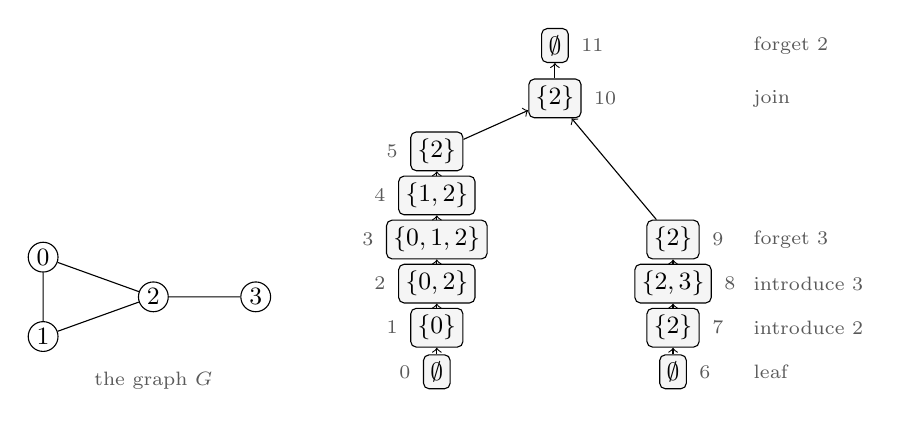
\begin{tikzpicture}[x=1cm,y=0.56cm,
  bag/.style={draw,rounded corners=2pt,inner sep=2.5pt,font=\small,fill=gray!8},
  lab/.style={font=\scriptsize,gray!70!black},
  v/.style={circle,draw,inner sep=1.2pt,font=\small,fill=white}]
  % the graph
  \node[v] (g0) at (-4.6,2.6) {0};
  \node[v] (g1) at (-4.6,0.8) {1};
  \node[v] (g2) at (-3.2,1.7) {2};
  \node[v] (g3) at (-1.9,1.7) {3};
  \draw (g0)--(g1)--(g2)--(g0) (g2)--(g3);
  \node[lab] at (-3.2,-0.2) {the graph $G$};
  % left branch (nodes 0..5)
  \foreach \i/\b/\y in {0/{$\emptyset$}/0, 1/{$\{0\}$}/1, 2/{$\{0,2\}$}/2, 3/{$\{0,1,2\}$}/3, 4/{$\{1,2\}$}/4, 5/{$\{2\}$}/5}
    { \node[bag] (a\i) at (0.4,\y) {\b}; \node[lab,left=1pt of a\i] {\i}; }
  % right branch (nodes 6..9)
  \foreach \i/\b/\y in {6/{$\emptyset$}/0, 7/{$\{2\}$}/1, 8/{$\{2,3\}$}/2, 9/{$\{2\}$}/3}
    { \node[bag] (a\i) at (3.4,\y) {\b}; \node[lab,right=1pt of a\i] {\i}; }
  \node[bag] (a10) at (1.9,6.2) {$\{2\}$}; \node[lab,right=1pt of a10] {10};
  \node[bag] (a11) at (1.9,7.4) {$\emptyset$}; \node[lab,right=1pt of a11] {11};
  \foreach \i/\j in {0/1,1/2,2/3,3/4,4/5,6/7,7/8,8/9,10/11} \draw[->] (a\i)--(a\j);
  \draw[->] (a5)--(a10); \draw[->] (a9)--(a10);
  % kinds
  \node[lab,anchor=west] at (4.3,0) {leaf};
  \node[lab,anchor=west] at (4.3,1) {introduce $2$};
  \node[lab,anchor=west] at (4.3,2) {introduce $3$};
  \node[lab,anchor=west] at (4.3,3) {forget $3$};
  \node[lab,anchor=west] at (4.3,6.2) {join};
  \node[lab,anchor=west] at (4.3,7.4) {forget $2$};
\end{tikzpicture}
\caption{A graph on four vertices and a nice tree decomposition of width~$2$, with the root at the top. The node numbers are the positions in the word of the decomposition: each node is written as its kind, its vertex, and, for the join node~$10$, its second child (node~$5$; its first child is the node just before it).}
\label{fig:nice}
\end{figure}


\section{The Two Theorems}

Both results are stated on the word RAM of the archive as follows. One program and one constant
serve every word length, every graph and every bound. They apply whenever the input fits with
room for $c\cdot 2^{c\ell^3}$ times a polynomial in its length, a condition checkable from the
input alone, and then the program halts within the stated number of instructions. The output is
either the word~$[0]$, admissible only when $G$ has no tree decomposition of width at most~$k$, or
the number~$1$ followed by the word of a nice tree decomposition of width at most~$k$. It is a
relation rather than a function, since a graph has many decompositions. The bounds are polynomial
in the encoded input length. The graph word has quadratic length in the number of vertices;
for the improvement theorem, the input also includes the supplied decomposition, whose size
is unrestricted. The formalized bounds are polynomial rather than linear in these lengths.

% lax begin Lax689794.BodlaenderKloks
\begin{theorem}[Bodlaender and Kloks~\cite{bodlaender1996efficient}]
\label{thm:bk}
Given a graph~$G$, a bound~$k$ and a nice tree decomposition of~$G$ of width at most~$\ell$, one can
decide whether $\tw(G)\le k$ and, if so, find a nice tree decomposition of width at most~$k$, in
time $2^{O(\ell^3)}\cdot\mathrm{poly}(N)$, where $N$ is the length of the complete encoded input, including the supplied decomposition.
\end{theorem}
% lax begin Lax689794Proofs.Fun.Final.improveDecomposition_proved
The exported proof uses the exact graph algorithm described below. If $\ell\le k$, it returns
the supplied decomposition. Otherwise it runs the graph algorithm with bound~$k$, independently
of the supplied decomposition. Since $k<\ell$, its parameter-dependent running time is bounded
by $2^{O(\ell^3)}$; reading and returning the supplied decomposition is covered by the polynomial
in the full input length.
% lax end
% lax end

% lax begin Lax689794.Bodlaender
\begin{theorem}[Bodlaender~\cite{bodlaender1996linear}]
\label{thm:bod}
Given a graph~$G$ and a bound~$k$, one can decide whether $\tw(G)\le k$ and, if so, find a nice
tree decomposition of~$G$ of width at most~$k$, in time $2^{O(k^3)}\cdot\mathrm{poly}(|G|)$.
\end{theorem}
% lax begin Lax689794Proofs.Fun.Final.niceDecomposition_computable_proved
The proof uses a dynamic program over characteristics of partial decompositions, following Althaus and Ziegler~\cite{althaus2020optimal}. Typical sequences describe the characteristics; introduce, forget and join transitions compute the tables, from which a decomposition is extracted. The vertices are inserted one at a time. Having a
nice decomposition of the graph on the first $i$ vertices, insert the next vertex into every bag.
This is a decomposition of the larger graph whose width has grown by one, and the improvement step
of this dynamic program brings the width back down to~$k$, or reports that the treewidth exceeds~$k$. The graph algorithm is proved first; the exported improvement theorem is then derived from it.
% lax end
% lax end

Done slightly differently than in the paper of Bodlaender, whose algorithm shrinks the graph by a
constant factor and recurses with linear running time, the algorithm formalized is the vertex by
vertex wrapper above. Its running time is $2^{O(k^3)}\cdot\mathrm{poly}$, which is what the
statement asks. Compression before conversion to a nice tree keeps the sizes of intermediate
decompositions polynomial in the graph size, with a parameter-dependent factor.

\section{How the Proofs Are Organized}

The proofs have two layers. The first proves correctness of the dynamic program on mathematical
objects, covering the sequences and their laws, decompositions as rooted trees with their bridges
to the archive's tree decompositions and to the word format, characteristics and their normal form,
the four kinds of node, and the tables. The second proves the running time. The Lean functions of
the first layer are run on a virtual machine for a first-order functional language whose semantics
carries a cost, a verified compiler takes that language to bytecode written in IMP+, and the
runs are transferred to the word RAM through the archive's compiler. Both theorems depend on Lean's
three standard axioms only.

\begin{thebibliography}{9}
\bibitem{althaus2020optimal} E.~Althaus and S.~Ziegler.
Optimal Tree Decompositions Revisited: A Simpler Linear-Time {FPT} Algorithm.
arXiv:1912.09144, 2020.
\bibitem{bodlaender1996linear} H.~L. Bodlaender.
A Linear-Time Algorithm for Finding Tree-Decompositions of Small Treewidth.
\emph{SIAM Journal on Computing}, 25(6):1305--1317, 1996.
\bibitem{bodlaender1996efficient} H.~L. Bodlaender and T.~Kloks.
Efficient and Constructive Algorithms for the Pathwidth and Treewidth of Graphs.
\emph{Journal of Algorithms}, 21(2):358--402, 1996.
\bibitem{kloks1994treewidth} T.~Kloks.
\emph{Treewidth: Computations and Approximations}.
Lecture Notes in Computer Science 842, Springer, 1994.
\end{thebibliography}
\end{document}
